
\section{Dasar Git} 
\noindent 
 \hspace*{0.5in} Git adalah $  $\textit{version control system} $  $yang digunakan para developer untuk mengembangkan software secara bersama-bersama. Fungsi utama git yaitu mengatur versi dari source code program anda dengan mengasih tanda baris dan code mana yang ditambah atau diganti. Git ini sebenernya memudahkan programmer untuk mengetahui perubahan source codenya daripada harus membuat file baru seperti $  $\textit{Program.java, ProgramRevisi.java, }\textit{ProgramRevisi2.java, ProgramFix.java}. Selain itu, dengan git kita tak perlu khawatir code yang kita kerjakan bentrok, karena setiap developer bias membuat branch sebagai $  $\textit{workspace}nya.Fitur yang tak kalah keren lagi, pada git kita bisa memberi komentar pada source code yang telah ditambah/diubah, hal ini mempermudah developer lain untuk tahu $  $ kendala apa yang dialami developer lain. \par
\noindent 
Untuk mengetahui bagaimana menggunakan git, berikut perintah-perintah dasar git: \par
\noindent 
\begin{enumerate}
\item Git init : untuk membuat $  $\textit{repository} $  $pada file lokal yang nantinya ada folder .git \par
\noindent 
\item Git status : untuk mengetahui status dari $  $\textit{repository} $  $lokal \par
\noindent 
\item Git add : menambahkan file baru pada $  $\textit{repository} $  $yang dipilih \par
\noindent 
\item Git commit : untuk menyimpan perubahan yang dilakukan, tetapi tidak ada perubahan pada $  $\textit{remote repository.} \par
\noindent 
\item Git push : untuk mengirimkan perubahan file setelah di commit ke $  $\textit{remote repository.} \par
\noindent 
\item Git branch : melihat seluruh $  $\textit{branch $  $}yang ada pada repository \par
\noindent 
\item Git checkout : menukar $  $\textit{branch $  $}yang aktif dengan $  $\textit{branch}yang dipilih \par
\noindent 
\item GIt merge : untuk menggabungkan $  $\textit{branch $  $}yang aktif dan $  $\textit{branch $  $}yang dipilih \par
\noindent 
\item Git clone : membuat Salinan $  $\textit{repository $  $}lokal\end{enumerate}
 \par
 \vspace{\baselineskip}
\noindent 
Contoh dari $  $\textit{software version control system} $  $adalah github, bitbucket, snowy evening, dan masih banyak lagi. Jika anda sebagai developer belum mengetahui fitur git ini, maka anda wajib mencoba dan memakainya. Karena banyak manfaat yang akan didapat dengan git ini. \par
\vspace{\baselineskip}
\noindent 
Git itu bukanlah sebuah bahasa seperti halnya HTML,CSS atau Js bukan pula sebuah konsep atau aturan baku dalam pemrograman, melainkan sebuah software yang berfungsi untuk mengatur source code dari aplikasi yang sedang anda buat. \par
\noindent 
Fungsi utamanya adalah untuk mengatur versi dari source code anda, menambahkan tanda/checkpoint ketika terjadi perubahan pada kode Anda dan tentunya akan mempermudah Anda untuk tetap mengetahui apa saja yang berubah dari source code Anda. \par
\vspace{\baselineskip}
\noindent 
Sebagai contoh, misalkan Anda sedang membangun sebuah website, dan anda akan menambahkan beberapa fitur dalam website anda. Agar tidak membingungkan nantinya anda membuat sebuah catatan terhadap apa yang telah anda lakukan seperti : \par
\noindent 
 \hspace*{0.5in} 01-04-2014 Memulai Project Website, File HTML  $  \&  $ CSS Dasar \par
\noindent 
 \hspace*{0.5in} 02-04-2014 Penambahan Menu Utama \par
\noindent 
 \hspace*{0.5in} 03-04-2014 Penambahan Layout Standar \par
\noindent 
 \hspace*{0.5in} 04-04-2014 Penambahan Fitur Pengubah Layout \par
 \vspace{\baselineskip}
\noindent 
 \hspace*{0.5in} Pada contoh diatas kita menggunakan tanggal sebagai tanda akan apa yang telah kita lakukan, dengan demikian kita bisa tahu kapan perubahan terjadi dan apa perubahan yang dilakukan. Dan dalam Git semua itu bisa dilakukan dengan mudah dan asyiknya jika Anda merusak kode sehingga membuat aplikasi error, maka anda dapat mengembalikan kode tersebut berdasarkan pada tanda/tanggal dimana kode masih normal, lebih mirip seperti restore point. \par
 \vspace{\baselineskip}
\noindent 
 \hspace*{0.5in} Git juga tidak hanya digunakan untuk perorangan, beberapa orang pun dapat bekerja secara bersamaan mengerjakan kode Anda dan Anda masih memiliki kontrol penuh terhadap kode Anda, Anda bisa menambahkan kode yang ditambahan oleh orang lain atau mengabaikannya sama sekali. oleh karena itu Git sering digunakan sebagai pengatur dalam projek kolaborasi dimana tidak hanya satu orang yang mengerjakan sebuah kode tapi beberapa orang sekaligus yang mengerjakan kode tersebut. \par
 \vspace{\baselineskip}
\noindent 
 \hspace*{0.5in} Git Punya Integritas \par
\noindent 
Segala sesuatu pada Git akan melalui proses checksum terlebih dahulu sebelum disimpan yang kemudian direferensikan oleh hasil checksum tersebut. Hal ini berarti tidak mungkin melakukan perubahan terhadap berkas manapun tanpa diketahui oleh Git. Fungsionalitas ini dimiliki oleh Git pada level terendahnya dan ini merupakan bagian tak terpisahkan dari filosofi Git. Anda tidak akan kehilangan informasi atau file yang tidak dimiliki oleh Git. \par
\vspace{\baselineskip}
\noindent 
 \hspace*{0.5in} Mekanisme checksum yang digunakan oleh Git adalah SHA-1 hash. Ini merupakan sebuah susunan string yang terdiri dari 40 karakter heksadesimal (0 sampai 9 dan a sampai f) dan dihitung berdasarkan bentuk dari suatu berkas atau struktur pada pada Git. sebuah hash SHA-1 seperti berikut: \par
 \vspace{\baselineskip}
\noindent 
Anda akan melihat seperti ini pada berbagai tempat di Git. Faktanya, Git tidak memiliki nama file pada basisdatanya, nilai hash dari isi berkas. \par
\vspace{\baselineskip}
\noindent 
Direktori Git adalah dimana Git menyimpan metadata dan database objek untuk projek anda. Ini adalah bahagian penting dari Git, dan inilah yang disalin saat anda melakukan kloning sebuah repositori dari komputer lain. \par
\vspace{\baselineskip}
\noindent 
Direktori kerja adalah sebuah checkout tunggal dari satu versi dari projek. File-berkas ini kemudian ditarik keluar dari basisdata yang terkompresi dalam direktori Git dan disimpan pada disk untuk anda pakai atau modifikasi. \par
\vspace{\baselineskip}
\noindent 
 \hspace*{0.5in} Alur kerja dasar Git adalah seperti ini: \par
\noindent 
 \hspace*{0.5in} Anda mengubah berkas dalam direktori kerja anda. \par
\noindent 
 \hspace*{0.5in} Anda membawa ke tahap, menambahkan snapshotnya ke area stage. \par
\noindent 
 \hspace*{0.5in} Anda melakukan komit \par
 \vspace{\baselineskip}
\noindent 
 \hspace*{0.5in} Aplikasi git dapat diakses melalui terminal/Command Prompt jadi silahkan buka Terminal/Command Prompt dan ketik $  $git --version $  $untuk melihat versi dari git yang terinstall dan untuk mengkonfirmasi jika proses instalasi berjalan mulus.  \par
 \vspace{\baselineskip}
 \vspace{\baselineskip}
\noindent 
Untuk mempelajari git ada baiknya kita buat sebuah studi kasus, pertama-tama kita buat folder baru untuk projek kita dan kita beri nama latihan-git. Anda bisa melakukannya melalui aplikasi Windows Explorer/File Manager/Finder namun kali ini untuk mengasah kemampuan Terminal/Command Promp Anda silahkan ketikkan perintah berikut: \par
\vspace{\baselineskip}
\noindent 
 \hspace*{0.5in} mkdir latihan-git \par
\noindent 
setelah folder latihan-git dibuat, kita navigasikan terminal ke dalam folder tersebut dengan mengetikkan peritah: \par
\vspace{\baselineskip}
\noindent 
 \hspace*{0.5in} cd latihan-git \par
 \vspace{\baselineskip}
 
 \begin{itemize}
 	\item File Status Lifecycle
 \end{itemize}
 
 \begin{figure}[ht]
 	\centerline{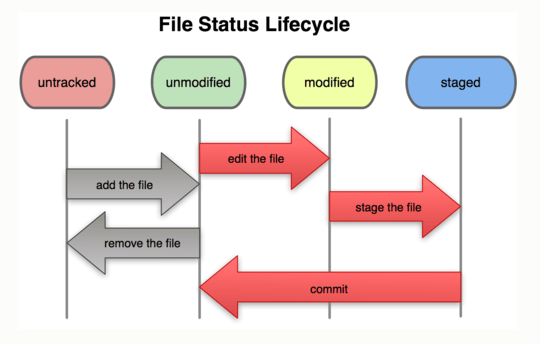
\includegraphics[width=0.70\textwidth]{figures/Git}}
 	\caption{File Status Lifecycle}
 	\label{File Status Lifecycle}
 \end{figure}
 
 
\noindent 
 \hspace*{0.5in} Git Init \par
\noindent 
Agar projek kita dapat diatur oleh git, maka kita perlu melakukan inisiasi git terlebih dahulu, caranya dengan mengetikkan perintah : \par
\vspace{\baselineskip}
\noindent 
 \hspace*{0.5in} git init \par
\noindent 
Perintah tersebut akan membuat folder .git dan didalamnya berisi file-file yang akan digunakan oleh Git untuk mengatur dan mengontrol project kita. \par
\vspace{\baselineskip}
\noindent 
 \hspace*{0.5in} Git Status \par
\noindent 
Untuk mengetahui status dari git, ketikkan perintah : \par
\vspace{\baselineskip}
\noindent 
 \hspace*{0.5in} git status \par
\noindent 
Anda akan mendapatkan keterangan seperti berikut: \par
\vspace{\baselineskip}
\noindent 
 \hspace*{0.5in} On branch master \par
\noindent 
 \hspace*{0.5in} Initial commit \par
\noindent 
 \hspace*{0.5in} nothing to commit (create/copy files and use "git add" to track) \par
\noindent 
Dari sana kita bisa mengetahui bahwa kita berada dalam branch master, dan kita telah melakukan initial commit, mengenai branch dan commit semuanya akan saya bahas nanti. \par
\noindent 
Sekarang mari kita buat file baru, misalkan buat file index.html lalu tambahkan kode berikut ke dalamnya \par
\begin{verbatim}
<!doctype html>
<html lang="en">
<head>
<meta charset="UTF-8"> 
<title>Belajar Git</title>
</head> 
<body> 
<p>Hello Git</p>
</body> 
</html> 
\end{verbatim}
\vspace{\baselineskip}
 \hspace*{0.5in} Git Add \par
\noindent 
Jika anda mengetikkan kembali perintah git status maka yang anda dapatkan kurang lebih seperti berikut : \par
\noindent 
On branch master~~~  \par
\noindent 
Initial commit \par
\noindent 
Untracked files: \par
\vspace{\baselineskip}
\noindent 
~  \hspace*{0.5in} (use "git add .." to include in what will be committed) \par
\noindent 
~~~  \hspace*{0.5in} index.html \par
\vspace{\baselineskip}
\noindent 
 \hspace*{0.5in} nothing added to commit but untracked files present (use "git add" to track) \par
\noindent 
Dari informasi diatas kita mendapatkan informasi bahwa Anda file baru yang belum terlacak. Kita perlu menambahkan file tersebut ke dalam git agar dapat dilacak perubahan-perubahan yang terjadi. Untuk itu anda dapat mengetikkan perintah: \par
\vspace{\baselineskip}
\noindent 
 \hspace*{0.5in} git add index.html \par
\noindent 
Dengan demikian anda telah menambahkan file index.html kedalam git agar bisa dimonitor/diawasi nantinya. Dan jika anda kembali mengetikkan git status yang akan anda dapatkan adalah: \par
\vspace{\baselineskip}
\noindent 
 \hspace*{0.5in} Changes to be committed: \par
\noindent 
 \hspace*{0.5in} ~~~ (use "git rm --cached .." to unstage) \par
\noindent 
 \hspace*{0.5in} ~~~~new~file:   index.html \par
 \vspace{\baselineskip}
\noindent 
 \hspace*{0.5in} Git Commit \par
\noindent 
Anda telah menambahkan file baru, namun anda belum melakukan commit. Oke, kembali ke contoh kasus dalam pembuka artikel ini, commit merupakan istilah untuk menandai terhadap perubahan yang telah anda lakukan, dalam contoh sebelumnya kita menandainya dengan tanggal dan keterangan singkat.  \par
\vspace{\baselineskip}
\noindent 
 \hspace*{0.5in} Nah untuk menandai setiap perubahan yang telah anda lakukan dan anda ingin agar git mengingatnya Anda harus melakukan commit terlebih dahulu. Untuk melakukan commit ketikkan perintah berikut: \par
 \vspace{\baselineskip}
\noindent 
 \hspace*{0.5in} git commit -m "Added index.html" \par
\noindent 
Dalam perintah diatas harus disertakan juga pesan commit, tanda -m digunakan untuk menambahkan pesan commit dan teks selanjutnya adalah pesan commit kita yakni  $ " $Added index.html $ " $. Jika semau anda lakukan dengan benar maka anda akan mendapatkan keterangan seperti berikut: \par
\vspace{\baselineskip}
\noindent 
 \hspace*{0.5in} [master (root-commit) 0181f7b] Added index.html \par
\noindent 
 \hspace*{0.5in}  1 file changed, 10 insertions(+) \par
\noindent 
 \hspace*{0.5in}  create mode 100644 index.html \par
\noindent 
 \hspace*{0.5in} Branch \par
 \vspace{\baselineskip}
\noindent 
Misalkan anda ingin menambahkan suatu fitur, namun anda tidak mau kode yang ada sekarang rusak karena fitur yang akan anda tambahkan masih belum stabil, Dalam Git anda dapat membuat branch terlebih dahulu. Branch ini bisa diartikan sebagai cabang dari branch master. segala perubahan yang anda lakukan pada branch yang anda buat tidak akan berpengaruh pada branch lainnya. \par
\noindent 
Sebagai contoh, kita buat branch dengan nama branch  $ " $fix-css $ " $ dengan mengetikkan perintah: \par
\vspace{\baselineskip}
\noindent 
 \hspace*{0.5in} git branch fix-css \par
 \vspace{\baselineskip}
\noindent 
Jika perintah dijalankan dengan benar maka ketika anda mengetikkan perintah git branch akan muncul branch-branch yang telah dibuat. \par
\vspace{\baselineskip}
\noindent 
 \hspace*{0.5in} ~~ fix-css \par
 \vspace{\baselineskip}
\noindent 
 \hspace*{0.5in} *~~ master \par
\noindent 
tanda Bintang menandakan bahwa anda sedang bekerja pada branch master, untuk berpindah ke branch yang baru saja dibuat (fix-css) ketikkan perintah berikut: \par
\vspace{\baselineskip}
\noindent 
 \hspace*{0.5in} git checkout fix-css \par
\noindent 
Jika peritah di atas benar, maka akan ada pemberitahuan seperti berikut: \par
\noindent 
 \hspace*{0.5in} Switched to branch 'fix-css' \par
 \vspace{\baselineskip}
\noindent 
\begin{itemize}
\item Github\end{itemize}
 \par
\noindent 
 \hspace*{0.5in} Github merupakan situs sharing code dan menggunakan git sebagai SCM-nya. Mungkin Anda pernah mendownload beberapa library/source code dari situs ini. Kini anda tahu mengapa kebanyakan source code dapat anda temui di github. \par
\vspace{12pt}
\noindent 
 \subsection{Apa itu GIT?} 
\noindent 
Git adalah version control, dengan menggunakan Git kita dapat menyimpan tiap perubahan yang kita lakukan pada file. Seperti menggunakan  $ " $undo $ " $ tetapi dapat digunakan pada seluruh file kita dan kita mempunyai log pada tiap perubahan yang kita simpan,  \par
\noindent 
Hal ini sangat berguna pada production environment, karena dengan adanya versioning, kita dapat dengan mudah melakukan rollback. Selain itu Git juga sangat membantu dalam proses pengembangan aplikasi. Salah satu platform Git yang terkenal adalah GitHub. Kita akan menggunakan GitHub untuk artiketl berikut. \par
\vspace{12pt}
\noindent 
\section{Repository}
\noindent 
Di Git Repository biasanya digunakan untuk mengorganisir sebuah projek. Projek dapat berisi files, folder, gambar, video dan lainnya yang dibutuhkan untuk sebuah project. Kami menyarankan untuk menambahkan file README yang bertujuan untuk memberi informasi terkait isi dari project tersebut. Kita dapat mengasumsikan Repository sebagai folder untuk menyimpan project kita. Satu berada di Local, dan yang satu berada di Remote disini kita menggunakan GitHub. \par
\vspace{\baselineskip}
\vspace{12pt}

{\fontsize{14pt}{14pt}\selectfont \textbf{Seperti Ini Perform Changes} \\} \par
\noindent 
 \hspace*{0.5in} Jerry mengkloning repositori dan memutuskan untuk menerapkan operasi string dasar. Jadi dia menciptakan file string.c. Setelah menambahkan isinya, string.c akan terlihat seperti berikut: \par
\vspace{12pt}
\noindent 
 \hspace*{0.5in}  $  \#  $include <stdio.h> \par
\noindent 
 \hspace*{0.5in} int my $  \_  $strlen (char * s) \hspace*{0.5in}  \par
\noindent 
 \hspace*{0.5in}  $  \{  $ \par
\noindent 
 \hspace*{0.5in}  $  $ $  $ $  $char * p = s; \par
\noindent 
 \hspace*{0.5in}  $  $ $  $ $  $sementara (* p) \par
\noindent 
 \hspace*{0.5in}  $  $ $  $ $  $ $  $ $  $ $  $++ p; \par
\noindent 
 \hspace*{0.5in}  $  $ $  $ $  $return (p - s); \par
\noindent 
 \hspace*{0.5in}  $  \}  $ \par
\noindent 
 \hspace*{0.5in} int main (void) \par
\noindent 
 \hspace*{0.5in}  $  \{  $ \par
\noindent 
 \hspace*{0.5in}  $  $ $  $ $  $int i; \par
\noindent 
 \hspace*{0.5in}  $  $ $  $ $  $char * s [] = \par
\noindent 
 \hspace*{0.5in}  $  $ $  $ $  $ $  \{  $ \par
\noindent 
 \hspace*{0.5in}  $  $ $  $ $  $ $  $ $  $ $  $"Git tutorial", \par
\noindent 
 \hspace*{0.5in}  $  $ $  $ $  $ $  $ $  $ $  $"Tutorial Point" \par
\noindent 
 \hspace*{0.5in}  $  $ $  $ $  $ $  \}  $; \par
\noindent 
 \hspace*{0.5in}  $  $ $  $ $  $untuk (i = 0; i <2; ++ i) $  $ $  $ $  $ $  $ $  $ $  $ \par
\noindent 
 $  $ $  $ $  $ \hspace*{0.5in} printf ("panjang string $  \%  $ s = $  \%  $ d  $  \setminus  $ n", s [i], my $  \_  $strlen (s [i])); \par
\noindent 
 \hspace*{0.5in}  $  $ $  $ $  $kembali 0; \par
\noindent 
 \hspace*{0.5in}  $  \}  $ \par
 \vspace{\baselineskip}
\noindent 
Dia menyusun dan menguji kodenya dan semuanya berjalan baik. Sekarang, dia bisa menambahkan perubahan ini ke repositori dengan aman. \par
\vspace{\baselineskip}
\noindent 
Git menambahkan operasi menambahkan file ke area stage. \par
\noindent 
 \hspace*{0.5in} [jerry @ CentOS project]  $  \$  $ git status -s \par
\noindent 
 \hspace*{0.5in} ?? tali \par
\noindent 
 \hspace*{0.5in} ?? string.c \par
\noindent 
 \hspace*{0.5in} [jerry @ CentOS project]  $  \$  $ git add string.c \par
 \vspace{\baselineskip}
\noindent 
Git menunjukkan tanda tanya sebelum nama file. Jelas, file-file ini bukan bagian dari Git, dan karena itulah Git tidak tahu apa yang harus dilakukan dengan file-file ini. Itu sebabnya, Git menunjukkan tanda tanya sebelum nama file. \par
\noindent 
Jerry telah menambahkan file ke area penyimpanan, perintah status git akan menampilkan file yang ada di area stage. \par
\vspace{\baselineskip}
\noindent 
 \hspace*{0.5in} [jerry @ CentOS project]  $  \$  $ git status -s \par
\noindent 
 \hspace*{0.5in} String.c \par
\noindent 
 \hspace*{0.5in} ?? tali \par
 \vspace{\baselineskip}
\noindent 
 \hspace*{0.5in} Untuk melakukan perubahan, dia menggunakan perintah komit git diikuti dengan opsi -m. Jika kita menghilangkan opsi -m. Git akan membuka text editor dimana kita bisa menulis multiline commit message. \par
 \vspace{\baselineskip}
\noindent 
 \hspace*{0.5in} [jerry @ CentOS project]  $  \$  $ git commit -m 'Implementasikan fungsi my $  \_  $strlen' \par
\noindent 
 \hspace*{0.5in} Perintah di atas akan menghasilkan hasil sebagai berikut: \par
\noindent 
 \hspace*{0.5in} [master cbe1249] Melaksanakan fungsi my $  \_  $strlen \par
\noindent 
 \hspace*{0.5in} 1 file berubah, 24 sisipan (+), 0 penghapusan (-) \par
\noindent 
 \hspace*{0.5in} buat mode 100644 string.c \par
 \vspace{\baselineskip}
\noindent 
Setelah berkomitmen untuk melihat rincian log, dia menjalankan perintah git log. Ini akan menampilkan informasi dari semua commit dengan commit komit mereka, commit author, commit date dan SHA-1 hash of commit. \par
\vspace{\baselineskip}
\noindent 
 \hspace*{0.5in} [jerry @ CentOS project]  $  \$  $ git log \par
 \vspace{\baselineskip}
\noindent 
Perintah di atas akan menghasilkan hasil sebagai berikut: \par
\noindent 
 \hspace*{0.5in} melakukan cbe1249b140dad24b2c35b15cc7e26a6f02d2277 \par
\noindent 
 \hspace*{0.5in} Penulis: Jerry Mouse <jerry@tutorialspoint.com> \par
\noindent 
 \hspace*{0.5in} Tanggal: Rabu Sep 11 08:05:26 2013 +0530 \par
\noindent 
 \hspace*{0.5in} Diimplementasikan fungsi my $  \_  $strlen \par
 \vspace{\baselineskip}
\noindent 
 \hspace*{0.5in}  \hspace*{0.5in} komit 19ae20683fc460db7d127cf201a1429523b0e319 \par
\noindent 
 \hspace*{0.5in}  \hspace*{0.5in} Penulis: Tom Cat <tom@tutorialspoint.com> \par
\noindent 
 \hspace*{0.5in}  \hspace*{0.5in} Tanggal: Rabu Sep 11 07:32:56 2013 +0530 \par
 \vspace{\baselineskip}
\noindent 
Komit awal \par
\noindent 
 \hspace*{0.5in} Jerry memeriksa versi terbaru dari repositori dan mulai mengerjakan sebuah proyek. Dia membuat file array.c di dalam direktori trunk. \par
 \vspace{\baselineskip}
 \vspace{\baselineskip}
\noindent 
 \hspace*{0.5in} [jerry @ CentOS  $  \sim  $]  $  \$  $ cd project $  \_  $repo / trunk / \par
\noindent 
 \hspace*{0.5in} [jerry @ CentOS trunk]  $  \$  $ cat array.c \par
\noindent 
 \hspace*{0.5in} Perintah di atas akan menghasilkan hasil berikut. \par
\noindent 
 \hspace*{0.5in}  $  \#  $include <stdio.h> \par
\noindent 
 \hspace*{0.5in}  $  \#  $define MAX 16 \par
\noindent 
 \hspace*{0.5in} int main (void)  $  \{  $ \par
\noindent 
 \hspace*{0.5in}  $  $ $  $ $  $int i, n, arr [MAX]; \par
\noindent 
 \hspace*{0.5in}  $  $ $  $ $  $printf ("Masukkan jumlah elemen:"); \par
\noindent 
 \hspace*{0.5in}  $  $ $  $ $  $scanf (" $  \%  $ d",  $  \&  $ n); \par
\noindent 
 \hspace*{0.5in}  $  $ $  $ $  $printf ("Enter the elements  $  \setminus  $ n"); \par
\noindent 
 \hspace*{0.5in}  $  $ $  $ $  $untuk (i = 0; i <n; ++ i) scanf (" $  \%  $ d",  $  \&  $ arr [i]); \par
\noindent 
 \hspace*{0.5in}  $  $ $  $ $  $printf ("Array memiliki elemen berikut  $  \setminus  $ n"); \par
\noindent 
 \hspace*{0.5in}  $  $ $  $ $  $untuk (i = 0; i <n; ++ i) printf (" $  \vert  $ $  \%  $ d  $  \vert  $", arr [i]); \par
\noindent 
 \hspace*{0.5in}  $  $ $  $ $  $printf (" $  \setminus  $ n"); \par
\noindent 
 \hspace*{0.5in}  $  $ $  $ $  $kembali 0; \par
\noindent 
 \hspace*{0.5in}  $  \}  $ \par
 \vspace{\baselineskip}
\noindent 
Dia ingin menguji kodenya sebelum melakukan. \par
\noindent 
 \hspace*{0.5in} [jerry @ CentOS trunk]  $  \$  $ buat array \par
\noindent 
 \hspace*{0.5in} cc array.c -o array \par
\noindent 
 \hspace*{0.5in} [jerry @ CentOS trunk]  $  \$  $ ./array \par
\noindent 
 \hspace*{0.5in} Masukkan jumlah elemen: 5 \par
\noindent 
 \hspace*{0.5in} Masukkan elemen \par
 \vspace{\baselineskip}
\noindent 
 \hspace*{0.5in}  \hspace*{0.5in} 1 \par
\noindent 
 \hspace*{0.5in}  \hspace*{0.5in} 2 \par
\noindent 
 \hspace*{0.5in}  \hspace*{0.5in} 3 \par
\noindent 
 \hspace*{0.5in}  \hspace*{0.5in} 4 \par
\noindent 
 \hspace*{0.5in}  \hspace*{0.5in} 5 \par
 \vspace{\baselineskip}
\noindent 
 \hspace*{0.5in} Array memiliki elemen berikut \par
\noindent 
 \hspace*{0.5in}  \hspace*{0.5in}  $  \vert  $ 1  $  \vert  $  $  \vert  $ 2  $  \vert  $  $  \vert  $ 3  $  \vert  $  $  \vert  $ 4  $  \vert  $  $  \vert  $ 5  $  \vert  $ \par
\vspace{12pt}
\vspace{\baselineskip}
\noindent 
Dia menyusun dan menguji kodenya dan semuanya berjalan seperti yang diharapkan, sekarang saatnya melakukan perubahan. \par
\vspace{\baselineskip}
\noindent 
 \hspace*{0.5in} [jerry @ CentOS trunk] status  $  \$  $ svn \par
\noindent 
 \hspace*{0.5in} ? array.c \par
\noindent 
 \hspace*{0.5in} ? array \par
 \vspace{\baselineskip}
\noindent 
Subversion menunjukkan '?' di depan nama file karena tidak tahu apa yang harus dilakukan dengan file-file ini. \par
\noindent 
Sebelum komit, Jerry perlu menambahkan file ini ke daftar perubahan yang tertunda. \par
\vspace{\baselineskip}
\vspace{\baselineskip}
\noindent 
 \hspace*{0.5in} [jerry @ CentOS trunk]  $  \$  $ svn tambahkan array.c \par
 \vspace{\baselineskip}
\noindent 
 \hspace*{0.5in} Sebuah array.c \par
 \vspace{\baselineskip}
\noindent 
Mari kita periksa dengan operasi 'status'. Subversion menunjukkan A sebelum array.c, artinya, file tersebut berhasil ditambahkan ke daftar perubahan yang tertunda. \par
\vspace{\baselineskip}
\noindent 
 \hspace*{0.5in} [jerry @ CentOS trunk] status  $  \$  $ svn \par
\noindent 
 \hspace*{0.5in} ? array \par
 \vspace{\baselineskip}
\noindent 
Sebuah array.c \par
\vspace{\baselineskip}
\noindent 
Untuk menyimpan file array.c ke repositori, gunakan perintah komit dengan opsi -m diikuti oleh pesan komit. Jika Anda menghilangkan opsi -m, Subversion akan menampilkan editor teks tempat Anda bisa mengetikkan pesan multi-baris. \par
\vspace{\baselineskip}
\noindent 
 \hspace*{0.5in} \vspace{12pt}
\noindent 
 \hspace*{0.5in} [jerry @ CentOS trunk]  $  \$  $ svn commit -m "Initial commit" \par
\noindent 
 \hspace*{0.5in} Menambahkan trunk / array.c \par
\noindent 
 \hspace*{0.5in} Mengirimkan data file \par
\noindent 
 \hspace*{0.5in} Komitmen revisi 2. \par
\noindent 
 \hspace*{0.5in} Sekarang file array.c berhasil ditambahkan ke repositori, dan nomor revisi bertambah satu. \par

